\RequirePackage{flashmovie}

\documentclass[mathserif,xcolor=dvipsnames]{beamer}
%\usepackage{pgfpages}
%\pgfpagesuselayout{4 on 1}[letterpaper,border shrink=5mm,landscape]

\usepackage{multimedia}

\usetheme{Warsaw}
\definecolor{PittBlue}{RGB}{0.61,0.73,0.35}
\usecolortheme[named=PittBlue]{structure}
\usepackage{beamerthemesplit}
\usepackage{amsmath}
\usepackage{amsfonts}
\usepackage{xcolor}
\usepackage{multimedia}
\usepackage{caption}
\usepackage{mdwlist}
\usepackage{pgf,pgfarrows,pgfnodes}
\usepackage{helvet}
\usefonttheme{structurebold}
\usepackage{hyperref}
\setbeamertemplate{navigation symbols}{}
\setbeamertemplate{footline}{}
\definecolor{myblue}{RGB}{0,20,70}
\definecolor{mypurple}{RGB}{102,0,204}
\definecolor{mygold}{RGB}{197,179,88}
\definecolor{mygreen}{RGB}{0,128,0}
\definecolor{myorange}{RGB}{255,204,0}
\definecolor{mydarkorange}{RGB}{252,108,0}

%\setbeamercolor{title}{fg=tugred}
%\setbeamercolor{frametitle}{fg=tugred}
%\setbeamercolor{boxesroundedtitle}{fg=white,bg=myblue}
%\setbeamercolor{item projected}{fg=white,bg=myblue}

\captionsetup{labelformat=empty,labelsep=none}
\def\Tiny{\fontsize{6pt}{6pt}\selectfont}
\renewcommand{\captionfont}{\Tiny}
\def\MediumFont{\fontsize{7pt}{7pt}\selectfont}

\definecolor{tugred}{rgb}{1.0,.04,.043}

\definecolor{tugblue}{rgb}{1.0,.04,.043}
%\definecolor{tugblue}{rgb}{0.31,0.51,0.74}


\definecolor{tuggreen}{rgb}{0.61,0.73,0.35}
\definecolor{tugmagenta}{rgb}{0.50,0.39,0.64}
\definecolor{tugorange}{rgb}{0.97,0.59,0.27}

\setbeamercolor{alerted text}{fg=tugblue}
\setbeamercolor*{palette primary}{fg=gray!60!black,bg=gray!30!white}
\setbeamercolor*{palette secondary}{fg=tugred!70!black,bg=gray!15!white}
\setbeamercolor*{palette tertiary}{bg=tugred!80!black,fg=gray!10!white}
\setbeamercolor*{palette quaternary}{fg=tugred,bg=gray!5!white}

\setbeamercolor*{sidebar}{fg=tugred,bg=gray!15!white}

\setbeamercolor*{palette sidebar primary}{fg=tugred!10!black}
\setbeamercolor*{palette sidebar secondary}{fg=white}
\setbeamercolor*{palette sidebar tertiary}{fg=tugred!50!black}
\setbeamercolor*{palette sidebar quaternary}{fg=gray!10!white}

\setbeamercolor*{titlelike}{parent=palette primary}
\setbeamercolor{titlelike}{parent=pallette primary,fg=white,bg=tugred}
\setbeamercolor{frametitle}{fg=white,bg=tugred}
\setbeamercolor{frametitle right}{bg=white}

\setbeamercolor*{separation line}{}
\setbeamercolor*{fine separation line}{}

\setbeamercolor{block title}{use=structure,fg=white,bg=tugblue}
\setbeamercolor{block title alerted}{use=alerted text,fg=white,bg=alerted text.fg!75!black}
\setbeamercolor{block title example}{use=example text,fg=white,bg=example text.fg!75!black}

\setbeamercolor{block body}{parent=normal text,use=block title,bg=block title.bg!10!bg}
\setbeamercolor{block body alerted}{parent=normal text,use=block title alerted,bg=block title alerted.bg!10!bg}
\setbeamercolor{block body example}{parent=normal text,use=block title example,bg=block title example.bg!10!bg}

\setbeamercolor{itemize item}{fg=tugblue}
\setbeamercolor{itemize subitem}{fg=tugblue}
\setbeamercolor{itemize subsubitem}{fg=tugblue}

%\setbeamercolor{section/subsection in toc}{fg=tugblue}
\setbeamercolor{section in toc}{fg=black,bg=white}
\setbeamercolor{subsection in toc}{fg=black,bg=white}

\setbeamercolor{structure}{fg=tugblue}

\setbeamertemplate{itemize subitem}{\rule{4px}{4px}}

%\mode<presentation>
{
%  \useoutertheme{default}   % empty
%  \useoutertheme{infolines}% simple but bland
 % \useoutertheme{split}    % ok if compress option used
%  \useoutertheme{shadow}   % way too much space used -- ok with option 'compress'
  %\useoutertheme{shadow}   
  %\setbeamercovered{transparent} % or whatever (possibly just delete it)
  %\useoutertheme[subsection=false]{miniframes}
}

\makeatletter
\setbeamertemplate{footline}
{
  \leavevmode%
  \hbox{%
  \begin{beamercolorbox}[wd=.3333\paperwidth,ht=2.25ex,dp=1ex,center]{author in head/foot}%
    \usebeamerfont{author in head/foot}%\insertshortauthor
    ~~\beamer@ifempty{\insertshortinstitute}{}{\insertshortinstitute}
  \end{beamercolorbox}%
  \begin{beamercolorbox}[wd=.3333\paperwidth,ht=2.25ex,dp=1ex,center]{title in head/foot}%
    \usebeamerfont{title in head/foot}\insertshorttitle
  \end{beamercolorbox}%
  \begin{beamercolorbox}[wd=.3333\paperwidth,ht=2.25ex,dp=1ex,right]{date in head/foot}%
%    \usebeamerfont{date in head/foot}\insertshortdate{}\hspace*{2em}
    \insertframenumber{} / \inserttotalframenumber\hspace*{2ex} 
  \end{beamercolorbox}}%
  \vskip0pt%
}
\makeatother



\makeatletter
\def\blfootnote{\xdef\@thefnmark{}\@footnotetext}
\makeatother


\usepackage{diagbox}


\setbeamertemplate{caption}{\raggedright\insertcaption\par}\newtheorem{conjecture}{Conjecture}[section]
\newtheorem{conj}{Conjecture}[section]
\newtheorem{question}{Question}[section]

\newtheorem{answer}{Answer}[section]
\newtheorem{exercise}{Exercise}[section]
\newtheorem{riddle}{Riddle}[section]


\newtheorem{remark}{Remark}[section]
\newtheorem{proposition}{Proposition}[section]
\newtheorem{assumption}{Assumption}[section]
\newtheorem{conditions}{Conditions}[section]
\newtheorem{tfram}{\hspace{0cm}}[section]

\usepackage{xcolor,soul}
\definecolor{lightblue}{rgb}{.90,.95,1}
\sethlcolor{lightblue}
\renewcommand<>{\hl}[1]{\only#2{\beameroriginal{\hl}}{#1}}

% http://tex.stackexchange.com/questions/41683/why-is-it-that-coloring-in-soul-in-beamer-is-not-visible
\makeatletter
\newcommand\SoulColor{%
  \let\set@color\beamerorig@set@color
  \let\reset@color\beamerorig@reset@color}
\makeatother
\SoulColor




\begin{document}



\frame{
\frametitle{\hspace{0cm}}


\begin{tfram}
\centering
The Newton-Gregory Problem
\end{tfram}
}

\frame{
\frametitle{Aristotle: On The Heavens (c. 350 B.C.)}

\begin{columns}[t]
\begin{column}{.50\textwidth}
\vspace{-1em}
\begin{question}
Is the regular icosahedron made of $\,20$ regular tetrahedra?
\end{question}
\vspace{0em}

\onslide<2,3>{
\noindent\rule[0.5ex]{\linewidth}{.5pt}
No! For circumradius $1,$ we can compute the edge length to be $$\Big(\frac{1}{2}\sqrt{\frac{1}{2}(5+\sqrt5)}\Big)^{-1}= 1.0514\dots.$$}


\end{column}



\begin{column}{.40\textwidth}
\vspace{-2em}
\centering
\begin{figure}[htbp] %  figure placement: here, top, bottom, or page
   \centering
   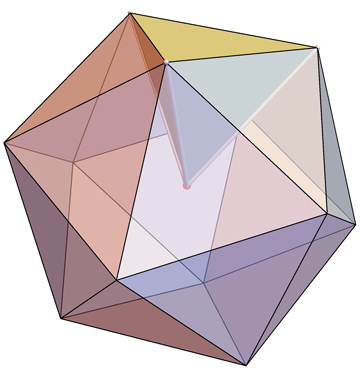
\includegraphics[width=1.9in]{imagesattalk/icosa.jpg} 
\end{figure}

\end{column}
\end{columns}
\onslide<3>{
\begin{riddle}\centering
Answer the question synthetically.
\end{riddle}}

}

\frame{
\frametitle{Aristotle: On The Heavens (c. 350 B.C.)}
\begin{remark}
\centering
If we place unit spheres at the vertices of that regular icosahedron, there is a lot of space between them.
\end{remark}
\begin{columns}[t]
\begin{column}{.40\textwidth}
\vspace{-3.5em}
\centering
\begin{figure}[htbp] %  figure placement: here, top, bottom, or page
   \centering
   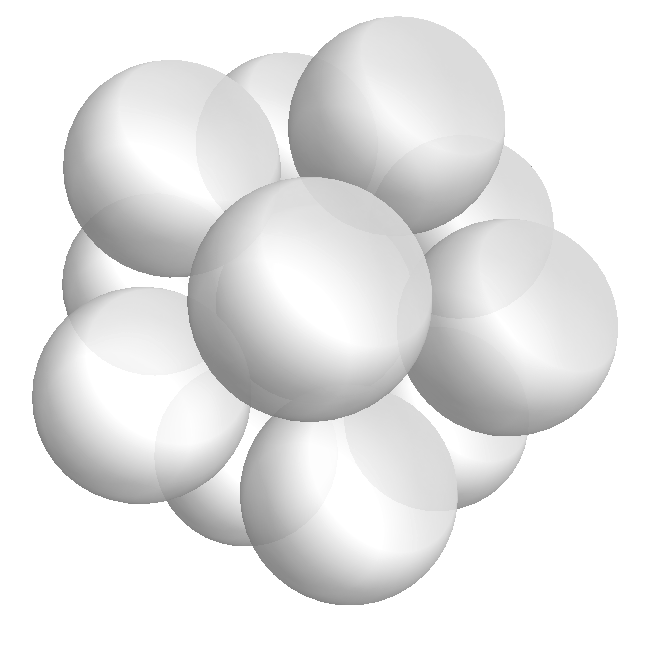
\includegraphics[width=1.9in]{imagesattalk/dod2.png} 
\end{figure}
\end{column}

\begin{column}{.40\textwidth}
\vspace{-3.5em}
\centering
\begin{figure}[htbp] %  figure placement: here, top, bottom, or page
   \centering
   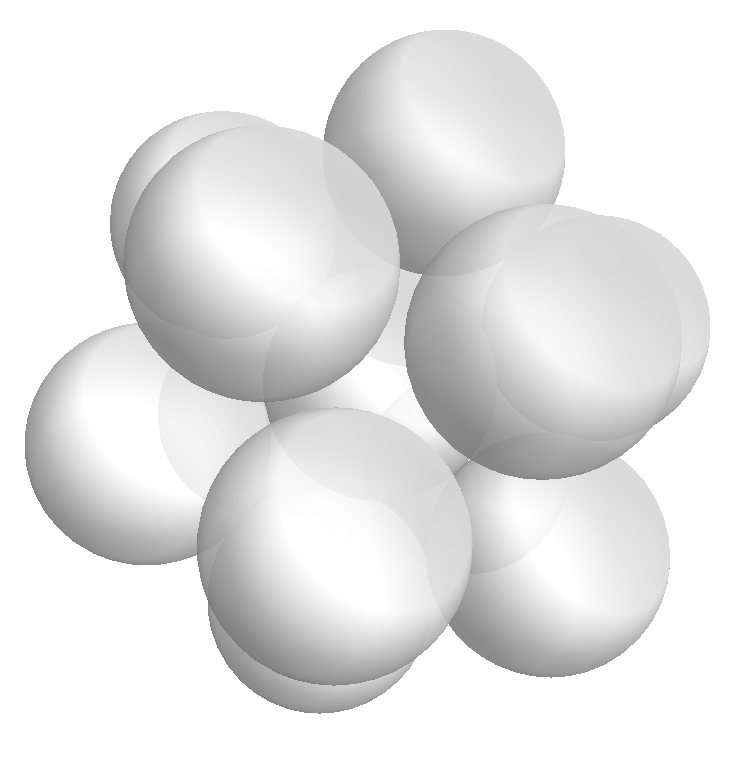
\includegraphics[width=1.9in]{imagesattalk/dod.png} 
\end{figure}
\end{column}
\end{columns}
\vspace{-.3cm}
\onslide<2>{
\begin{question}[Newton-Gregory]
\centering
Can we fit in a thirteenth sphere?
\end{question}}

}



\frame{
\frametitle{Newton and Gregory: Principia (revision c. 1694)}

\begin{columns}[t]
\begin{column}{.40\textwidth}
\vspace{-3.5em}

\centering
\begin{figure}[htbp] %  figure placement: here, top, bottom, or page
   \centering
   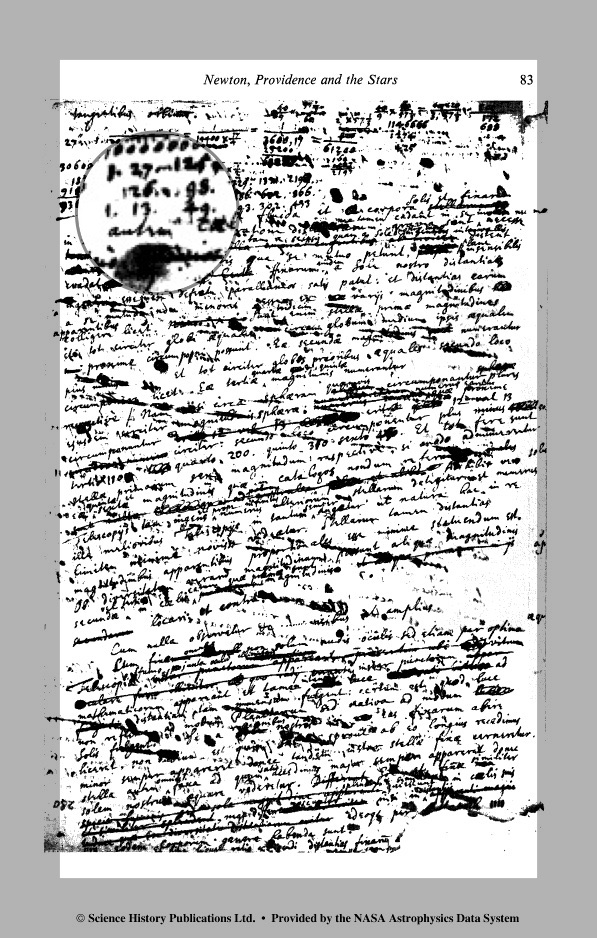
\includegraphics[width=1.9in]{imagesattalk/t2png} 

\end{figure}
\end{column}


\begin{column}{.55\textwidth}
%\vspace{-.75cm}
%\begin{question}
%how many non-overlapping unit spheres could be placed in contact with a central unit sphere?
%\end{question}\hspace{1cm}

For Newton and Gregory, this was a problem of mechanics:  
Why the fixed stars don't all fall into the sun. \newline 

In a draft for the second edition of \emph{Principia}, Newton considers stars of various magnitudes as modeled by arrangements of equal balls.\newline

This method was abandoned, but history lends the names of Newton and Gregory to the problem.
\end{column}
\end{columns}

}

\frame{
\frametitle{Kepler: Epitome Astronomiae Copernicanae (c. 1620)}

\begin{columns}[t]
\begin{column}{.40\textwidth}
\vspace{-3.5em}

\centering
\begin{figure}[htbp] %  figure placement: here, top, bottom, or page
   \centering
   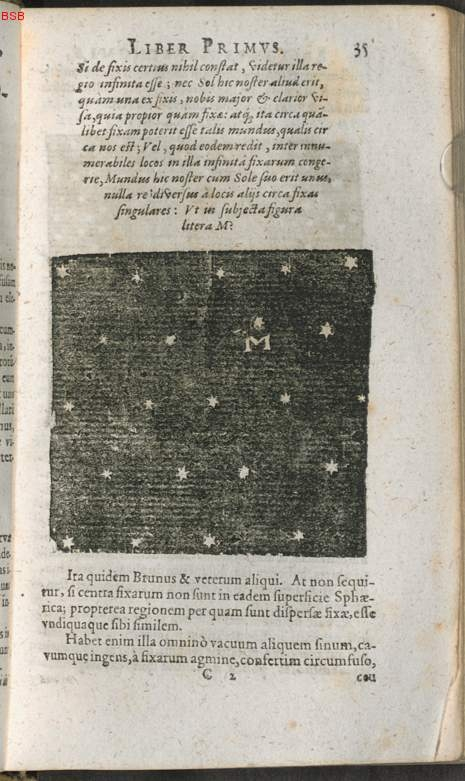
\includegraphics[width=1.9in]{imagesattalk/wasserzeichen-projekte1.jpeg} 

\end{figure}
\end{column}

\begin{column}{.40\textwidth}
\vspace{-3.5em}
\centering

\begin{figure}[htbp] %  figure placement: here, top, bottom, or page
   \centering
   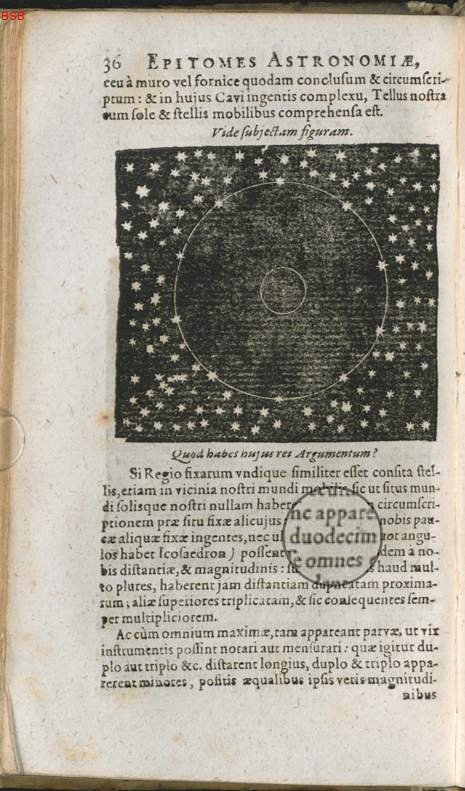
\includegraphics[width=1.9in]{imagesattalk/wasserzeichen-projekte2.jpeg} 

\end{figure}
\end{column}
\end{columns}
}
%He also refers to Brunus, Giordano Bruno, who was burned at the stake 20 years prior.



\frame{
\frametitle{Naive Bound}

\begin{columns}[t]
\begin{column}{.50\textwidth}
We know some good ways to arrange $12$ spheres to touch a central one.
\newline
\noindent\rule[0.5ex]{\linewidth}{.5pt}
There is a bound given by the solid angle.
Centrally projecting to the surface of the central sphere, this region has area
$$2\pi(1-\cos{\frac{\pi}{6}}) = .26\dots$$
giving a bound of
$$\frac{4\pi} {2\pi(1-\cos{ \frac{\pi}{6}})} =14.9\dots.$$

\end{column}




\begin{column}{.40\textwidth}
\only<1>{
\begin{figure}[htbp] %  figure placement: here, top, bottom, or page
   \centering
   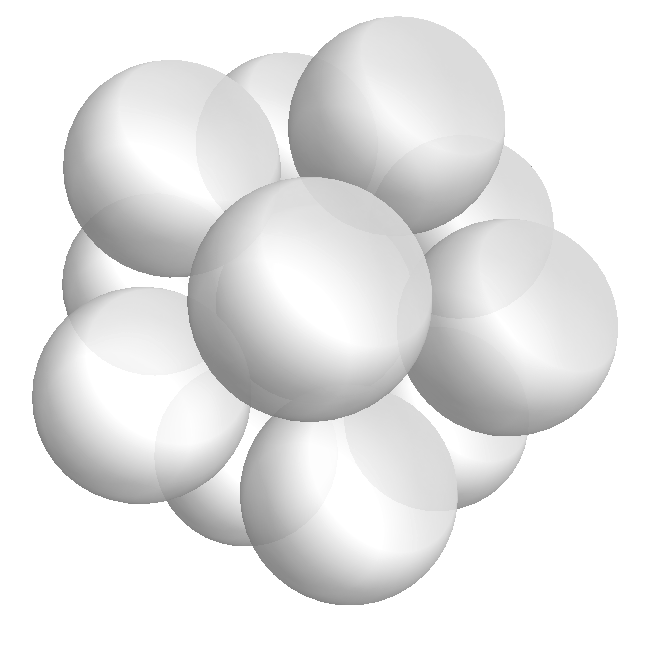
\includegraphics[width=1.9in]{imagesattalk/dod2.png} 
\end{figure}}
\only<2>{
\begin{figure}[htbp] %  figure placement: here, top, bottom, or page
   \centering
   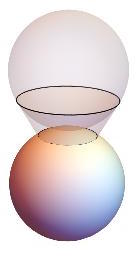
\includegraphics[width=1.3in]{imagesattalk/solidangle} 
\end{figure}}

\end{column}
\end{columns}

}

\frame{
\frametitle{Less Naive Bound}
\begin{columns}[t]
\begin{column}{.47\textwidth}
\vspace{1em}
\centering
Triangulate the contacts.
\begin{figure}[htbp] %  figure placement: here, top, bottom, or page
   \centering
   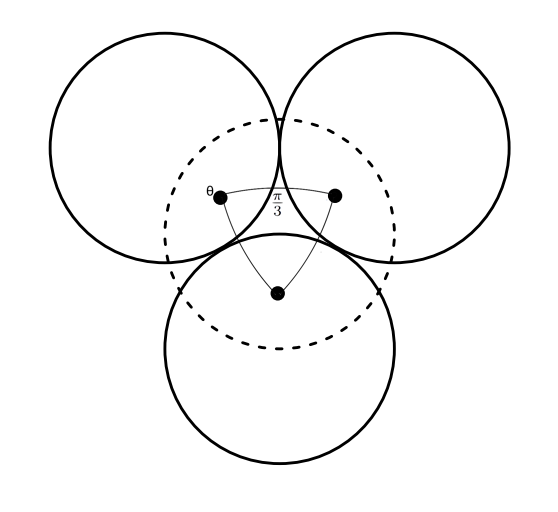
\includegraphics[width=1.5in]{imagesattalk/trianglecontact} 
\end{figure}
\vspace{-1.5em}
\onslide<2,3,4>{
\begin{assumption}
 Good triangulations exist and the area minimizer is the face of a regular tetrahedron. 
\end{assumption}}
\end{column}

\begin{column}{.50\textwidth}
\onslide<3,4>{From Euler characteristic:

$v-e+f=2$ and $3\hspace{-.1em}f = 2e$ for triangulations of the sphere, giving $f = 2v -4.$\newline

The minimal face area is $$T:=3\arccos{(\frac{1}{3}) - \pi}= 0.55\dots.$$
\onslide<4>{
Then for $v= 13$
$$4\pi - 22 * T = 0.43...$$
but for $v= 14$  
$$4\pi - 24 * T = -0.66\dots.$$}}
\end{column}
\end{columns}
}




\frame{
\frametitle{Bender, Hoppe (c. 1874)}
\begin{columns}[t]
\begin{column}{.40\textwidth}
\vspace{-3em}
\centering
\begin{figure}[htbp] %  figure placement: here, top, bottom, or page
   \centering
   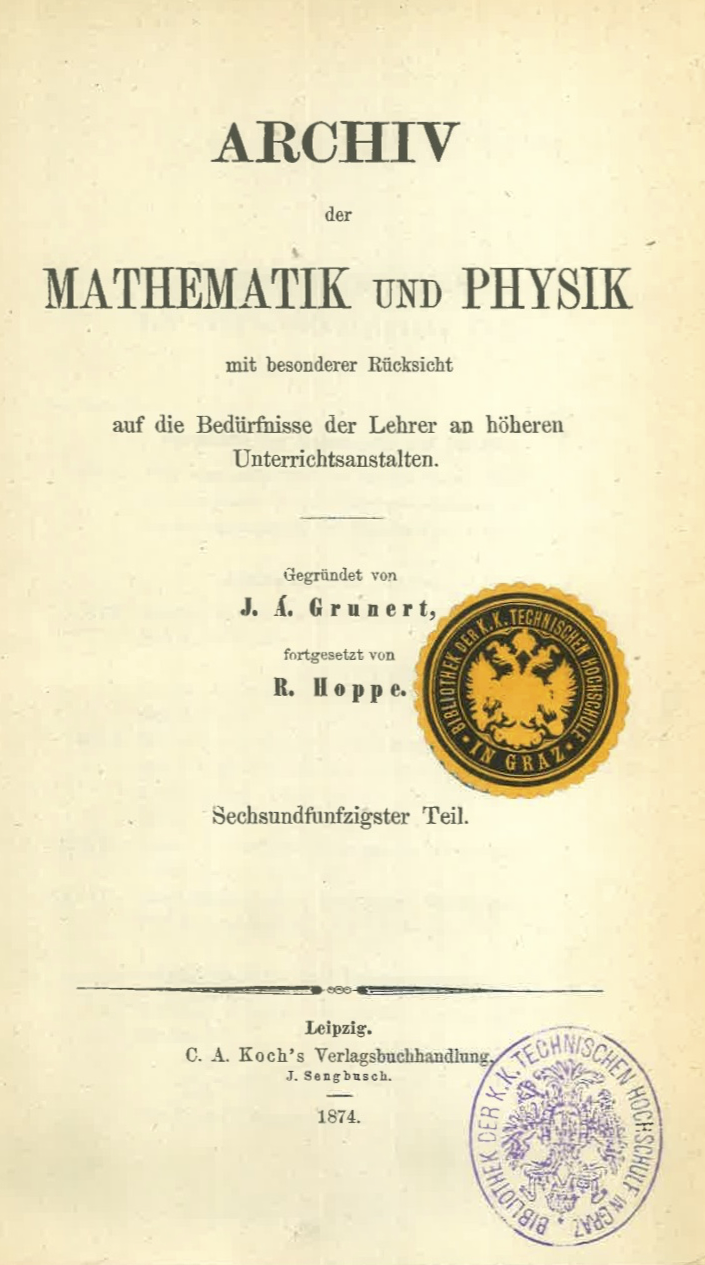
\includegraphics[width=1.5in]{imagesattalk/Bender} 
\end{figure}
\end{column}

\begin{column}{.50\textwidth}
\centering
\vspace{-3em}
\centering
\begin{figure}[htbp] %  figure placement: here, top, bottom, or page
   \centering
   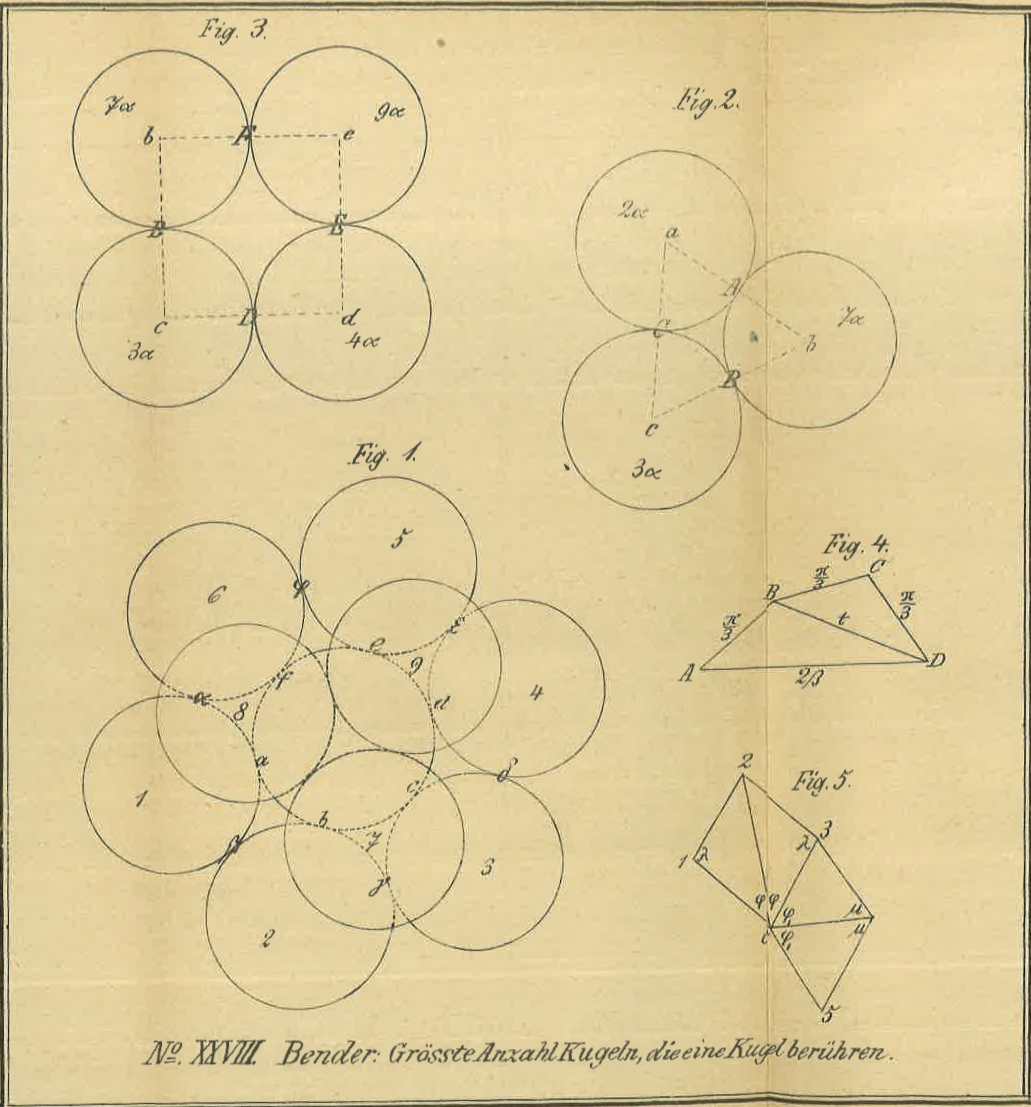
\includegraphics[width=1.9in]{imagesattalk/Bender2} 
\end{figure}

Contact graphs: geometric graphs with a vertex for each kissing sphere and edges recording contact.
\end{column}
\end{columns}
}



\frame{
\frametitle{Sch\"utte and van der Waerden, Leech (c. 1950)}

\begin{columns}[t]
\begin{column}{.50\textwidth}

Sch\"utte and van der Waerden further analyzed such graphs and gave conditions on the contact graph showing that $13$ unit spheres touching a central unit sphere would induce a graph that was not realizable.

\end{column}

\begin{column}{.50\textwidth}

\centering

Using similar techniques, Leech gave a proof consisting of only two pages.  Much of this brevity seems to come from \newline

\begin{quote}certain details which are tedious rather than difficult being omitted.\end{quote}
\end{column}
\end{columns}
\onslide<2>{
\begin{theorem}[Sch\"utte and van der Waerden]
\centering
We can only fit twelve spheres. 
\end{theorem}}
}


\frame{
\frametitle{\hspace{0cm}}
\begin{tfram}
\centering
The Tammes Problem
\end{tfram}
}


\frame{
\frametitle{P. M. L. Tammes (1930)}
\begin{columns}[t]
\begin{column}{.6\textwidth}
\vspace{-.5cm}
\begin{question}What is the maximal radius possible for $\,N$ equal spheres, all touching a central sphere of radius $\,1$?\end{question}
Another formulation of the \emph{Tammes problem}: How many spherical caps of angular diameter $\theta$ that can be placed without overlap? \newline\newline
\onslide<2,3>{
Tammes was studying pollen grains and empirically determined $6$ for $\theta = \frac{2\pi}{4}$ but no more than $4$ for $\theta > \frac{2\pi}{4}$.  }
\end{column}
\begin{column}{.3\textwidth}
\centering
\vspace{-1cm}
\begin{figure}[htbp] %  figure placement: here, top, bottom, or page
   \centering
   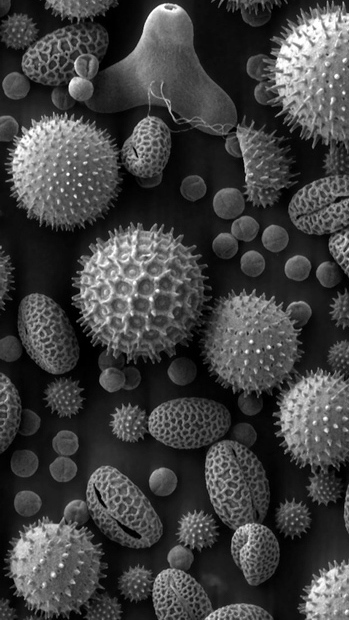
\includegraphics[width=1.3in]{imagesattalk/pollen} 
   \end{figure}
\end{column}
\end{columns}
\onslide<3>{\begin{remark}
\centering The maximizing configuration for $5$ is not unique.\end{remark}}

}

\frame{
\frametitle{L. Fejes-T\'{o}th (1943)}

The Tammes problem was solved for $N= 3, 4, 6$ and $12$, with configurations of cap centers for $N=3$ attained by vertices of an equatorial equilateral triangle and for $N=\{4, 6, 12\}$ by vertices of regular tetrahedron, octahedron and icosahedron. \begin{figure}[htbp] %  figure placement: here, top, bottom, or page
   \centering
      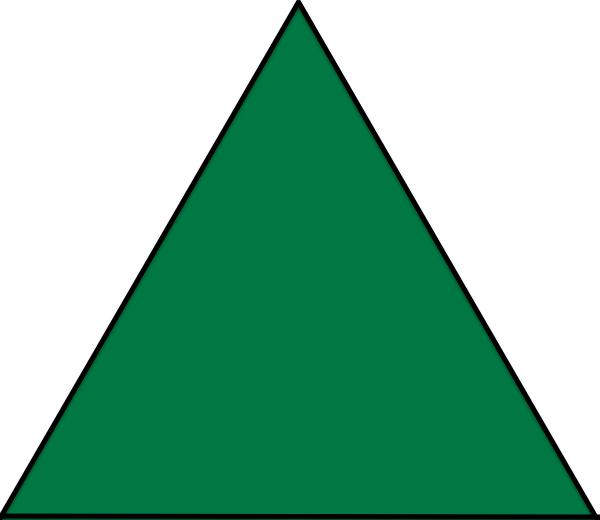
\includegraphics[width=1in]{imagesattalk/tri1.png} 
   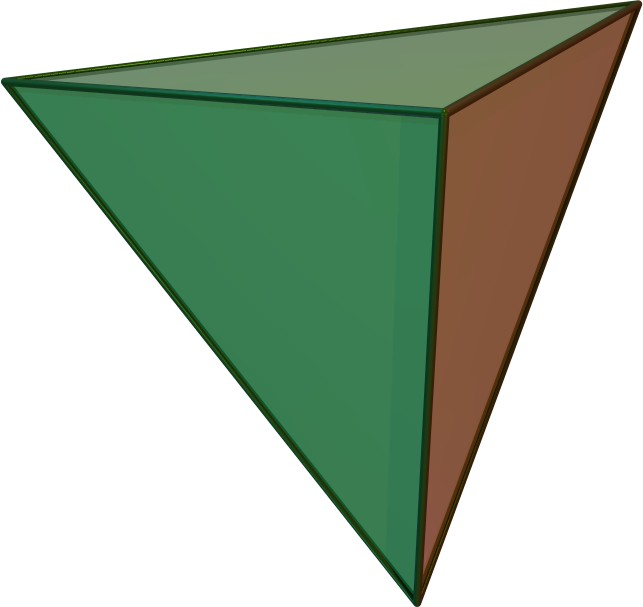
\includegraphics[width=1in]{imagesattalk/tet1.jpg} 
    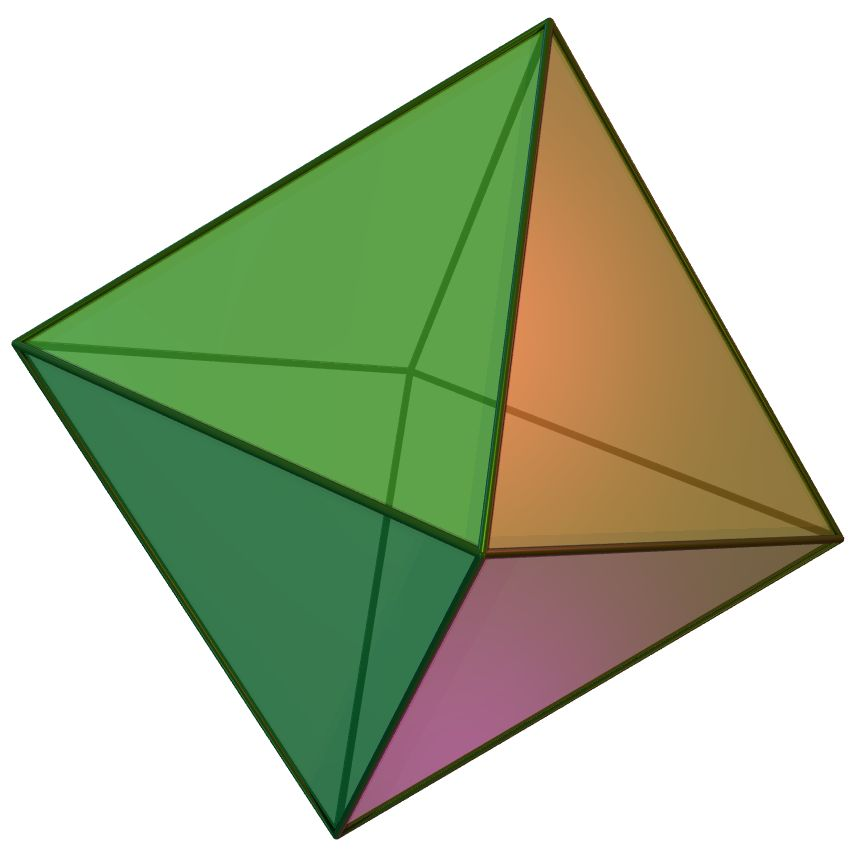
\includegraphics[width=1in]{imagesattalk/oct1.jpg} 
     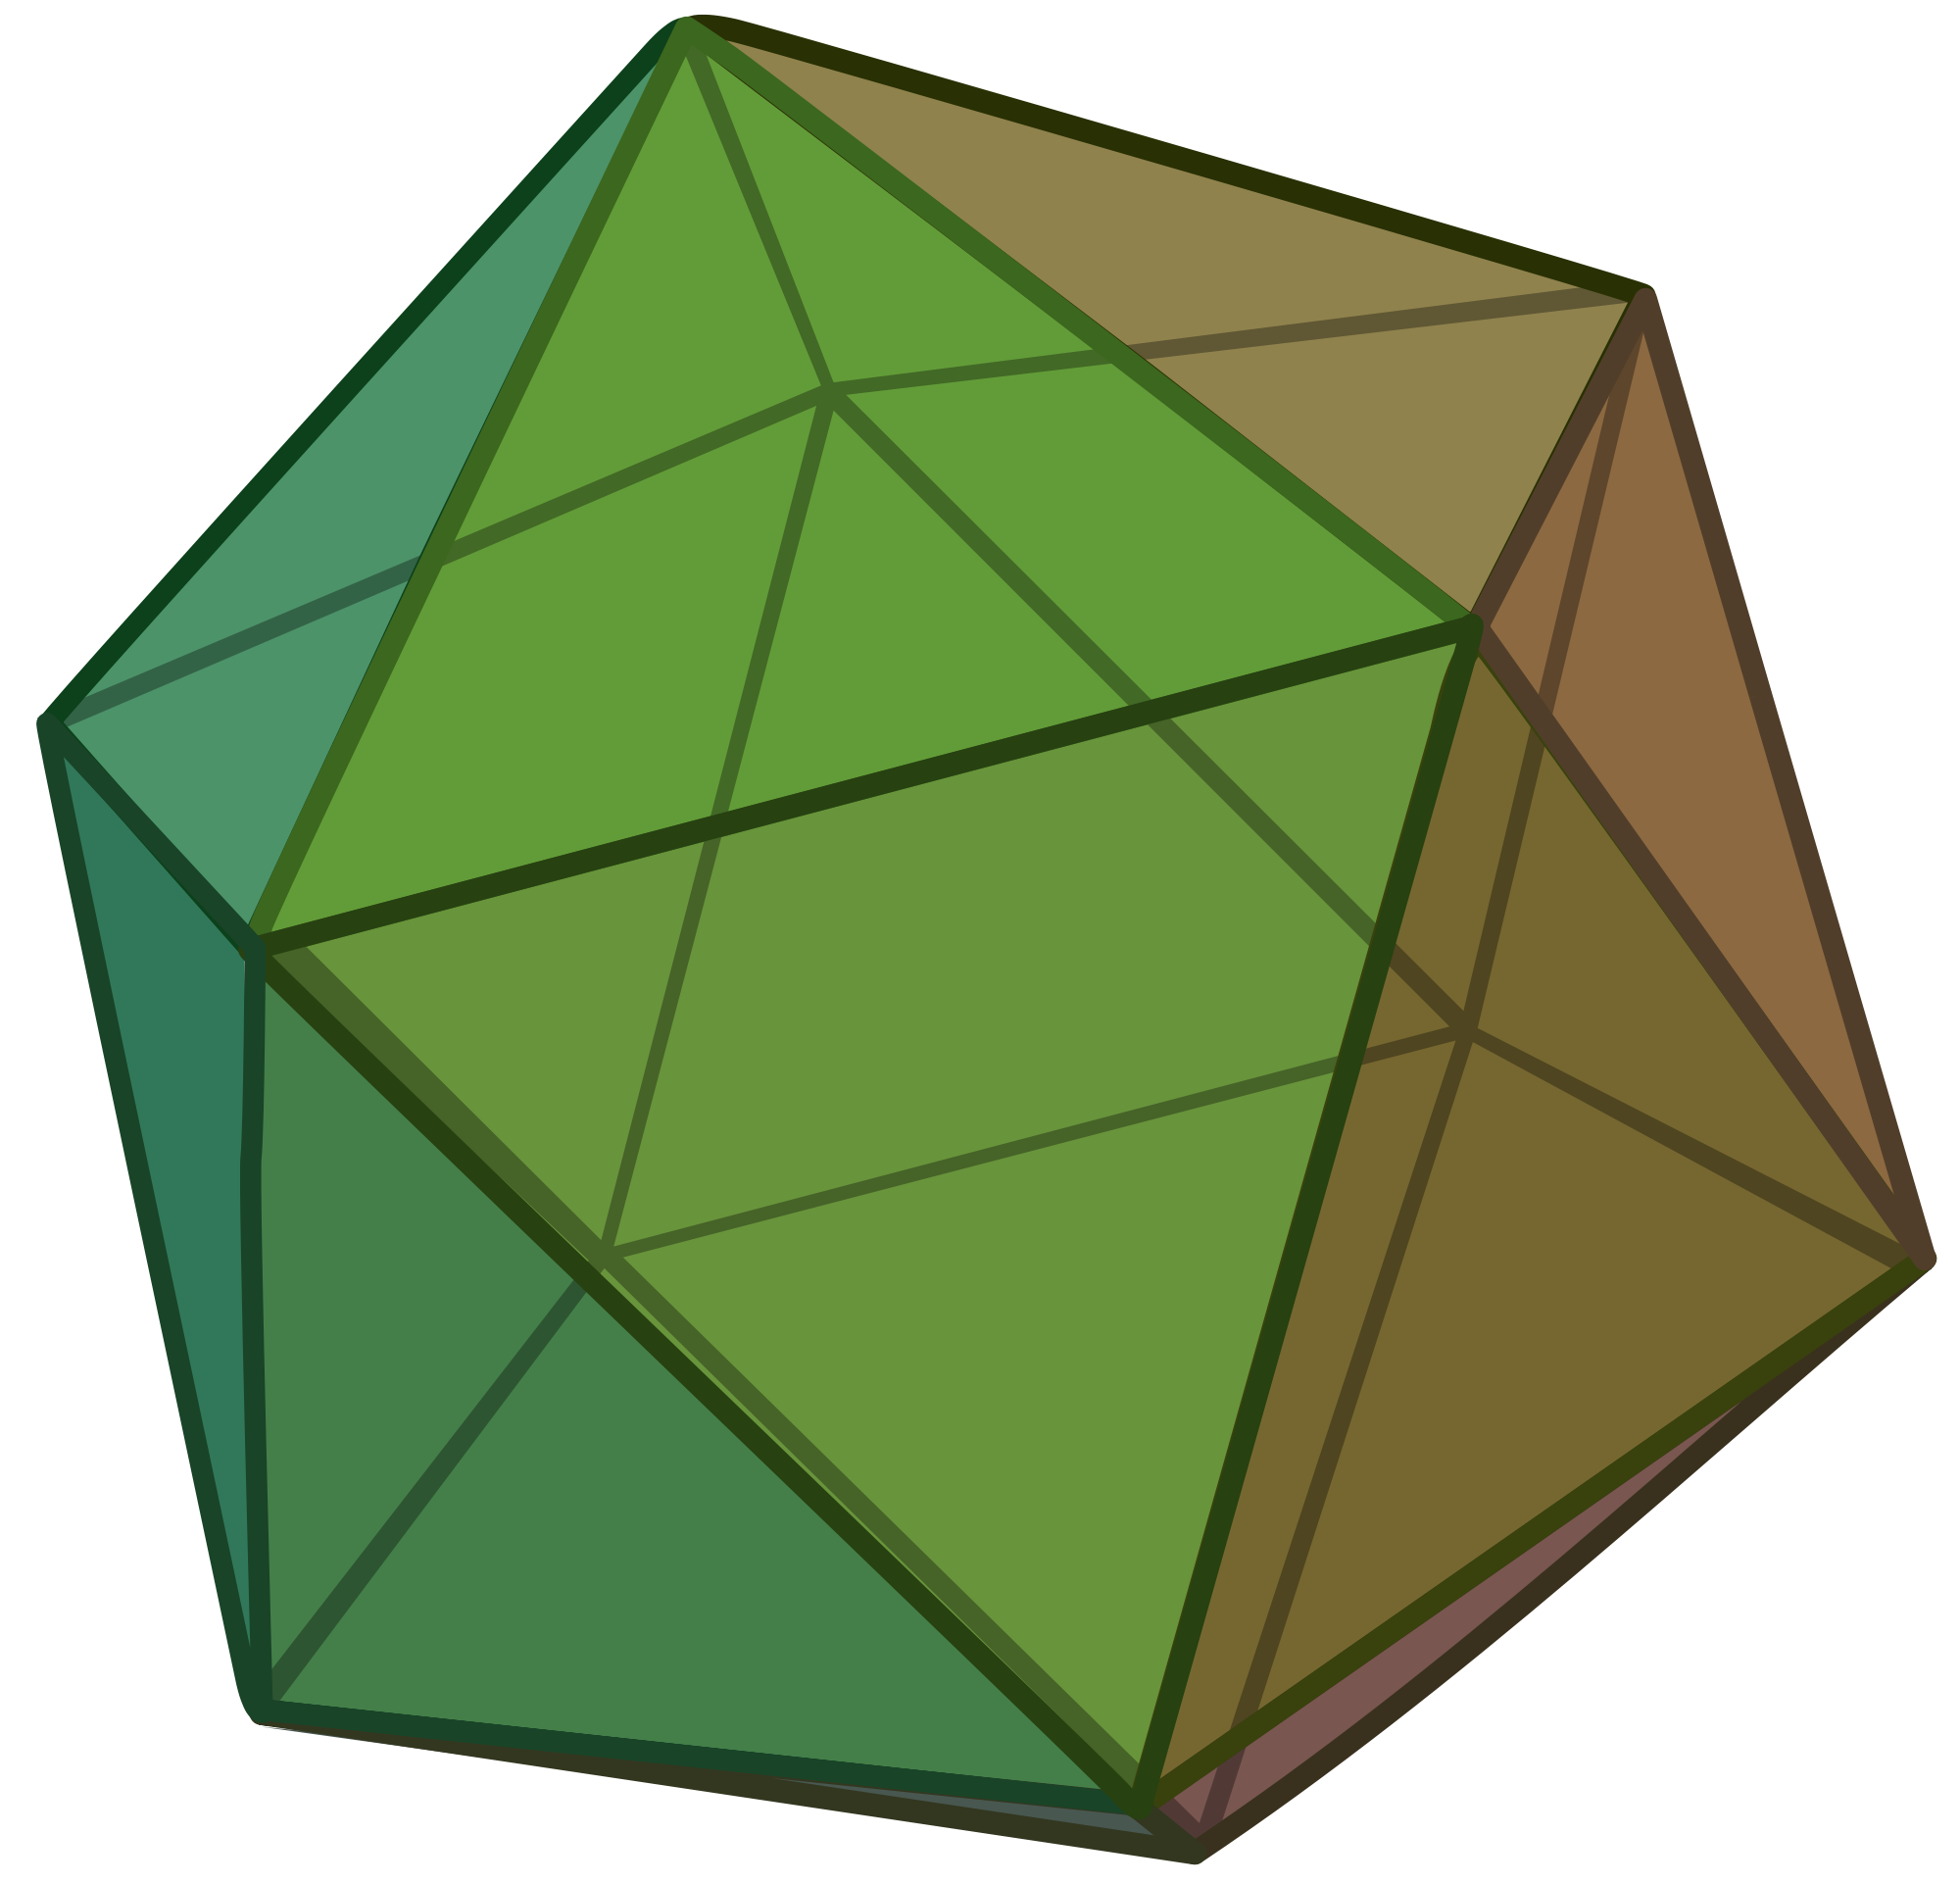
\includegraphics[width=1in]{imagesattalk/ico1.png} 
   

\end{figure}

}

\frame{
\frametitle{L. Fejes-T\'{o}th (1943)}
Fejes-T\'{o}th proved the inequality\newline \begin{theorem}
for $\,N$ points on the sphere, there are $\,2$ with angular distance
\[
\theta \le \arccos \Big( \frac{ (\cot (\omega)^2 -1}{2}\Big), \quad \omega = \Big(\frac{N}{N-2} \Big) \frac{\pi}{6}.
\]
\end{theorem}\hspace{0cm}
The inequality is sharp for $N=\{3, 4, 6, 12\}$. 

\onslide<2>{
\begin{remark}
$\theta$ is the edge length of a equilateral spherical triangle with the expected area for an element of an $N-$vertex triangulation.
\end{remark}}


%\begin{riddle}\centering
%Prove the Lexell circle theorem using intuitive geometry
%\end{riddle}

}
%\frame{
%\frametitle{L. Fejes-T\'{o}th (1943)}
%\begin{theorem}
%The maximum radius of $12$ equal spheres touching a central sphere of radius $1$ is:
%
%\[
%r(12) = \frac{1}{\sqrt{\frac{5+ \sqrt{5}}{2}} -1} = 1.1085...,
%\]
%
%a real root of a fourth degree polynomial equation  $$x^4 -6x^3 +x^2+4x+1.$$
%
%An extremal configuration achieving this radius is given by the vertices of an inscribed regular icosahedron; equivalently, the centers of faces of a circumscribed regular dodecahedron.
%\end{theorem}
%}
%

\frame{
\frametitle{\hspace{0cm}}
\begin{columns}[t]
\begin{column}{.50\textwidth}
The Tammes problem has been solved exactly for only $3 \le N \le 14$ and $N=24$. It was solved for $N=\{5, 7, 8, 9\}$ by Sch\"{u}tte and van der Waerden in 1951, $N=\{10, 11\}$ by Danzer in his 1963 Habilitationsschrift. 
\vspace{.5cm}
\begin{figure}[htbp] %  figure placement: here, top, bottom, or page
   \centering
     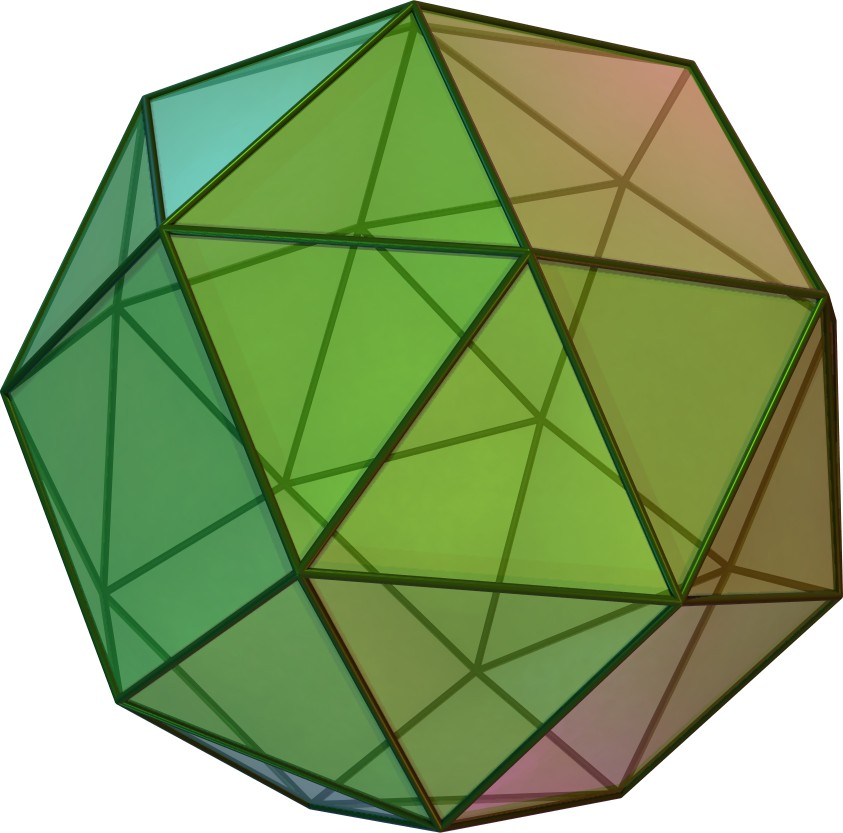
\includegraphics[width=1in]{imagesattalk/snub1.jpg} 
\end{figure}

\end{column}
\begin{column}{.5\textwidth}
\vspace{-.5cm}
\begin{figure}[htbp] %  figure placement: here, top, bottom, or page
   \centering
   \hspace{-2em}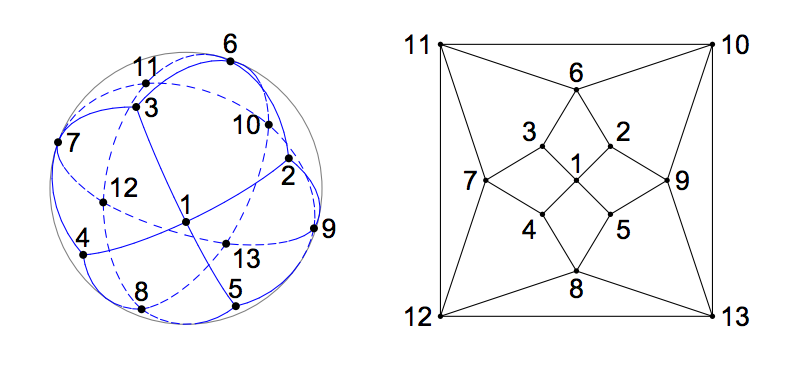
\includegraphics[width=2in]{imagesattalk/musin.png} 
\end{figure}\vspace{-1em}
$N=24$ was solved by Robinson in 1961 showing the configuration of centers were the vertices of a snub cube.  Recently the Tammes problem was solved for the cases $N=\{13, 14\}$ by Musin and Tarasov by generating all candidate contact graphs.
\end{column}
\end{columns}



}



\frame{
\frametitle{Approximate Values}
\tiny
 \begin{table}[h]
 \centering
\renewcommand{\arraystretch}{.70}
%formerly .85
\begin{tabular}{|r|c|l|l|l|}
\hline &&&&\\[-.7em]
\multicolumn{1}{|c|}{$N$} &
\multicolumn{1}{c|}{$\theta(N)$}&
\multicolumn{1}{c|}{$r_{max}(N)$}&
\multicolumn{1}{c|}{Configuration}&
\multicolumn{1}{c|}{Source}\\    [.3em]\hline&&&&\\[-.7em]
3 &      $\delta_3=\frac{2\pi}{3}= 120^{\circ}$   &\vtop{\hbox{\strut  $ 3+ 2 \sqrt{3}$ }\hbox{\strut  $\approx 6.4641$}} & Equilateral Triangle & Fejes-T\'{o}th (1943)   \\
   [.3em]\hline &&&&\\[-.7em]
 4 &    \vtop{\hbox{\strut\hspace{1.75em}  $\delta_4=\cos^{-1}(-\frac{1}{3})$ \quad}\hbox{\strut\hspace{3.25em}$\approx 109.4712^{\circ}$}}  &   \vtop{\hbox{\strut $ 2+ \sqrt{6}$ }\hbox{\strut $\approx 4.4495$}} & Regular Tetrahedron & Fejes-T\'{o}th (1943) \\
   [.3em] \hline&&&&\\[-.7em]
 5 &     $\delta_5=\frac{2 \pi}{4}  = 90^{\circ}$ &  \vtop{\hbox{\strut$1+\sqrt{2}$}\hbox{\strut$\approx 2.4142$ }}    &   \vtop{\hbox{\strut Regular Octahedron }\hbox{\strut minus one vertex }}    &  Fejes-T\'{o}th (1943)\\
 %$\approx 2.41421$
    [.3em] \hline&&&&\\[-.7em]
 6 &     $\delta_6  =\frac{2 \pi}{4} = 90^{\circ}$ &  \vtop{\hbox{\strut$1+\sqrt{2}$}\hbox{\strut$\approx 2.4142$ }}   & Regular Octahedron & Fejes-T\'{o}th (1943)  \\
%$\approx 2.41421$
   [.3em] \hline&&&&\\[-.7em]
 7 &    $\delta_7 \approx 77.8695^{\circ}$  &$\approx 1.6913$ & [No name] &  \vtop{\hbox{\strut Schutte and}\hbox{\strut van der Waerden (1951) }}   \\
   [.3em]\hline&&&&\\[-.7em]
 8 &    $\delta_8 \approx 74.8585^{\circ}$ & $\approx 1.5496$ & Square Antiprism & \vtop{\hbox{\strut Schutte and}\hbox{\strut van der Waerden (1951) }}  \\
 \hline&&&&\\[-.7em]
 9 &     $\delta_9 \approx 70.5288^{\circ}$ &\vtop{\hbox{\strut  $\frac{1+\sqrt{3}}{2}$}\hbox{\strut $ \approx 1.3660$ }}  & [No name] & \vtop{\hbox{\strut  Schutte and}\hbox{\strut  van der Waerden (1951) }}  \\
   [.3em]\hline&&&&\\[-.7em]
 10 &     $\delta_{10} \approx 66.1468^{\circ}$ & $\approx 1.2013$ &  [No name]  & Danzer (1963) \\
 [.3em] \hline&&&&\\[-.7em]
 11&     $\delta_{11} \approx 63.4349^{\circ}$ &  \vtop{\hbox{\strut $ \frac{1}{\sqrt{\frac{5+ \sqrt{5}}{2}} -1}$}\hbox{\strut $\approx 1.1085$}}  & \vtop{\hbox{\strut Regular Icosahedron}\hbox{\strut minus one vertex}} &Danzer (1963)  \\
 %$\approx 1.10851$
   [.3em] \hline&&&&\\[-.7em]
  12&     $\delta_{12}  \approx 63.4349^{\circ}$    &  \vtop{\hbox{\strut $ \frac{1}{\sqrt{\frac{5+ \sqrt{5}}{2}} -1}$}\hbox{\strut $\approx 1.1085$}}   & Regular Icosahedron & Fejes-T\'{o}th (1943) \\
 % $\approx 1.10851$
  [.3em]  \hline&&&&\\[-.7em]
  13 &   $\delta_{13}\approx 57.1367^{\circ}$   & $\approx 0.9165 $ & [No name ]  & Musin and Tarasov (2013) \\
  % $\approx 0.91649$
   [.3em] \hline&&&&\\[-.7em]
14 &    $\delta_{14} \approx 55.6706^{\circ}$  & $\approx 0.8759$ & [No name]  & Musin and Tarasov (2015)  \\
% $ \approx 0.87593$
    [.3em]\hline&&&&\\[-.7em]
24 &     $\delta_{24}\approx 43.6908^{\circ}$ &   $\approx 0.5926$   & Snub Cube & Robinson
(1961) \\
%$\approx 0.59262$
   [.3em]
\hline
\end{tabular}
\end{table}
}





\frame{
\frametitle{\hspace{0cm}}
\centering
\begin{tfram}
\centering
Configuration Spaces
\end{tfram}
}


\frame{
\frametitle{Variable Radii}

\begin{definition}
$\operatorname{Conf}(N,r)$ is the configuration space of $N$ non-intersecting balls of radius $r$ on the sphere.  (Equivalently, caps of radius $\theta.$)
\end{definition}
\begin{itemize}
\item For $r$ small, $\operatorname{Conf}(N,r) \simeq \textrm{Conf}(N,0).$
\item For $r$ large,  $\operatorname{Conf}(N,r)= \emptyset.$

\end{itemize}
\begin{remark}The Tammes problem is equivalent to finding the maximal $r$ such that $\operatorname{Conf}(N,r)$ is non-empty.  
\end{remark}

\begin{remark}
The result for $N=13$ gives a solution to Newton-Gregory.
\end{remark}
}


\frame{
\frametitle{Critical radii}


\begin{columns}[t]\vspace{-2em}
\begin{column}{.60\textwidth}
There are certain radii that are critical in the sense of (stratified) Morse Theory:  The topology of the configuration space changes.  
\newline

These radii also correspond to configurations of points that are force balanced:  There exists a non-trivial strut measure on the contact graph that force balances all the vertices.
\onslide<2>{
\begin{remark}
Such configurations obstruct the $r$-subgradient flow, which normally can be used to define a strong deformation retraction.
\end{remark}}

\end{column}

\begin{column}{.40\textwidth}

\begin{figure}[htbp] %  figure placement: here, top, bottom, or page
   \centering
   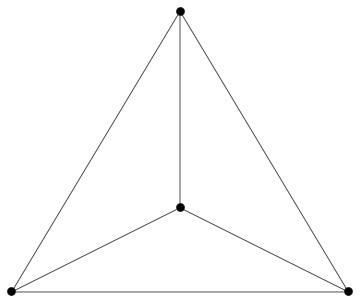
\includegraphics[width=1in]{imagesattalk/n4.jpg} 

\end{figure}

\begin{figure}[htbp] %  figure placement: here, top, bottom, or page
   \centering
   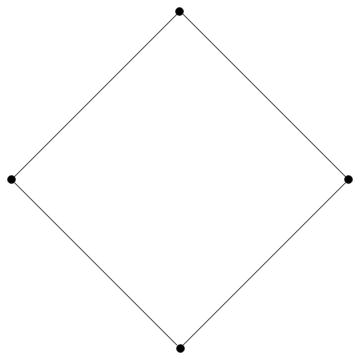
\includegraphics[width=1in]{imagesattalk/graph4.jpg} 

\end{figure}

\end{column}
\end{columns}



}


\frame{
\frametitle{Critical radii}


\begin{theorem}
To each critical value $\theta$ for the radius, there is a force balanced configuration. 
\end{theorem}


\begin{theorem}
There are a finite number of critical values for
the radius function.
\end{theorem}

\onslide<2,3>{
\begin{remark}
From this, it is pretty clear that the notion of criticality is one sided.  And the Morse theoretic picture is not so nice.  But for small $N$, we can really understand the configuration space.  
\end{remark}
}

\onslide<3>{
\begin{riddle}
Draw a cartoon for $N=3$.
\end{riddle}}

}


\frame{
\frametitle{Critical radii for 4 points}


\begin{columns}[t]
\begin{column}{.50\textwidth}

For $4$ points, we have
\begin{itemize}

\item$0\le \theta<\frac{2\pi}{4}:$ $$\operatorname{Conf}(4,r(\theta))\simeq \textrm{Conf}(n,0)$$

\item$\frac{2\pi}{4} < \theta\le \arccos{(-\frac{1}{3})}:$  $$\operatorname{Conf}(4,r(\theta))\simeq \{0,1\}$$

\item$\theta>\arccos{(-\frac{1}{3})}:$  $$\operatorname{Conf}(4,r(\theta))= \emptyset$$

\end{itemize}




\end{column}

\begin{column}{.5\textwidth}


\begin{figure}[htbp] %  figure placement: here, top, bottom, or page
   \centering
   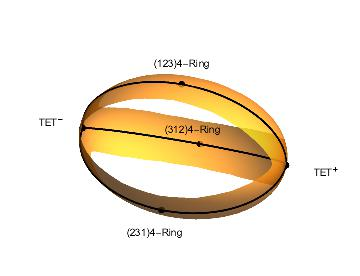
\includegraphics[width=2in]{imagesattalk/morse.jpg} 

\end{figure}

\end{column}
\end{columns}



}








\frame{
\frametitle{Betti Numbers}

Betti numbers for configuration space $\operatorname{Conf}(N,0)/SO(3)$ can be computed.

\begin{table}[h]
\tiny
\renewcommand{\arraystretch}{0.9}
\begin{center}
	\begin{tabular}{| c | r |r | r| r | r |r |r|r|r|r|}
	\hline
	\backslashbox{\raisebox{.5mm}{$N$}}{\raisebox{-1mm}{$k$}}  &  $0$ & $1$ & $2$ & $3$ & $4$ & $5$ & $6$  & $7$ & $8$ \\ \hline &&&&&&&&&\\[-.7em]
	        $3$ & $1$ &$0$ & $0$ & $0$ & $0$ & $0$ & $0$ & $0$ & $0$ \\
	$4$ & $1$ &$2$ &$0$ & $0$ & $0$ & $0$ & $0$ & $0$ &  $0$ \\
	$5$ & $1$ &$5$ &$6$ & $0$ & $0$ & $0$ & $0$ & $0$ & $0$  \\
	$6$ & $1$ &$9$ &$26$ & $24$ & $0$ & $0$ & $0$  & $0$ & $0$ \\
	$7$ & $1$ &$14$ &$71$ & $154$ & $120$ & $0$  & $0$ & $0$ & $0$ \\
	$8$ & $1$ &$20$ &$155$ & $580$ & $1044$ & $720$   & $0$ & $0$ & $0$ \\
        $9$ & $1$ &$27$ &$295$ & $1665$ & $5104$ & $8028$   & $5040$ & $0$ & $0$ \\
        $10$ & $1$ &$35$ &$511$ & $4025$ & $18424$ & $48860$    & $69264$ & $40320$ & $0$ \\
        $11$ & $1$ & $44$ & $826$ & $8624$ & $54649$ & $214676$ & $509004$ & $663696$ & $362880$\\

	\hline
	\end{tabular}
\end{center}
\end{table}


}



\frame{
\frametitle{Critical radii for 4 points}

The Euler characteristic of our the configuration space is $\chi(\operatorname{Conf}(4,0))/SO(3))=-1$.  

Using the indexed sum of critical points of the function $\rho: \operatorname{Conf}(4,0)/SO(3) \rightarrow \mathbb{R}$ gives an alternative computation 
$$\chi(\operatorname{Conf}(4,0)/SO(3)) = \sum _k (-1)^k  \# (\,\textrm{critical points of co-index = } k \, ).
$$

Since the $4$-Ring has symmetry group $D_4$ of order $8$ in $SO(3)$, there are $3=|S_4/D_4|$ critical points of this type with co-index $1$; and since TET has symmetry group $A_4$ of order $12$ in $SO(3)$,
there are really $2=|S_4/A_4|$ critical points of this type with co-index $0$
 \[
 \chi(\operatorname{Conf}(4,0)/SO(3))=2-3=-1
 \]

}



\frame{
\frametitle{5 points: the highest stratum}

In general, the structure of the critical points are not nice.

\begin{figure}[htbp] %  figure placement: here, top, bottom, or page
   \centering
 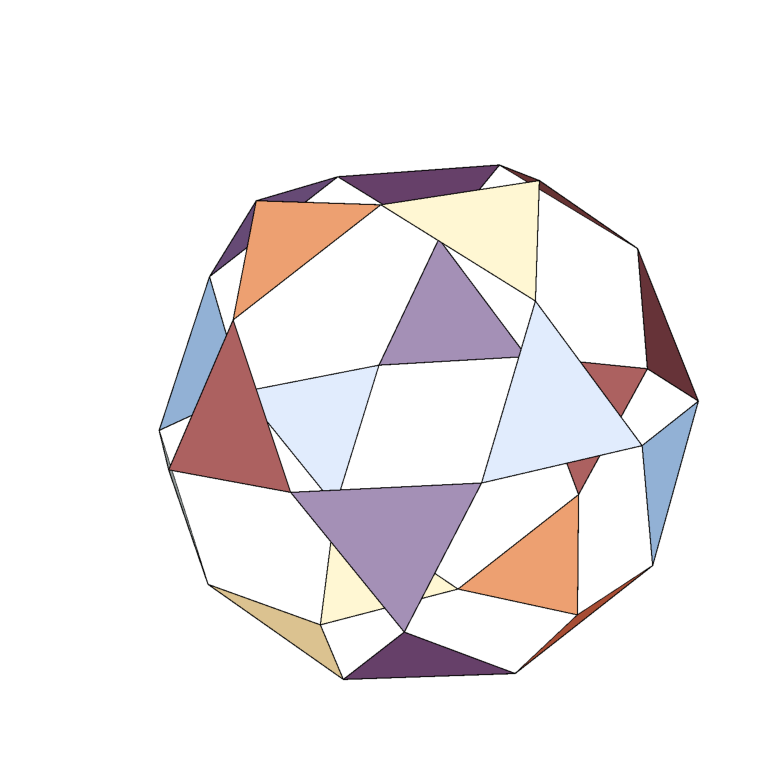
\includegraphics[width=2in]{imagesattalk/complex.pdf} 
\end{figure}

}

\frame{
\frametitle{12 points: Frederick Charles Frank}



\begin{columns}[t]
\begin{column}{.6\textwidth}
\onslide<1,2>{

Frank argued that the supercooling of liquids can occur because the common arrangements of molecules in liquids assumes configurations far from what they would assume if frozen.\newline }

\onslide<2>{
He claimed that there are exactly $3$ configurations of $12$ unit spheres next to a given central sphere: The FCC configuration, the HCP configuration, and the dodecahedral configuration. 
\end{column}

\begin{column}{.40\textwidth}
\centering

\vspace{-.7cm}
\begin{figure}[htbp] %  figure placement: here, top, bottom, or page
   \centering
      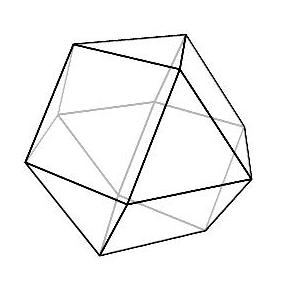
\includegraphics[width=.8in]{imagesattalk/fccskel.jpg}\\
      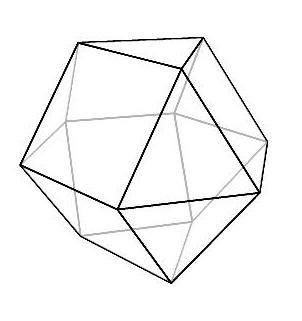
\includegraphics[width=.8in]{imagesattalk/hcpskel.jpg}\\
           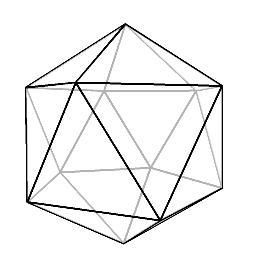
\includegraphics[width=.8in]{imagesattalk/icoskel2.jpg}
\end{figure}
}


\end{column}
\end{columns}
}






\frame{
\frametitle{\hspace{1em}}

`` Consider the
question of how many different ways one can put twelve billiard balls in
simultaneous contact with another one, counting as different the arrangements
\ul{which cannot be transformed into each other} without breaking contact with
the centre ball?' \hl{The answer is {\em three}. Two which come to the mind
of any crystallographer occur in the face-centred cubic and hexagonal close
packed lattices. The third comes to the mind of any good schoolboy, and it
is to put one at the center of each face of a regular dodecahedron.}
That body has five-fold axes, which are abhorrent to crystal symmetry:
unlike the other two packings, this one cannot be continuously extended in
three dimensions. You will find that the outer twelve in this packing do not
touch each other.''\\
\hspace{2in}--- Frederick Charles Frank
}


\frame{
\frametitle{The Jitterbug}
\begin{columns}[t]
\begin{column}{.5\textwidth}
\centering

\only<1>{
\begin{figure}[htbp] %  figure placement: here, top, bottom, or page
   \centering
   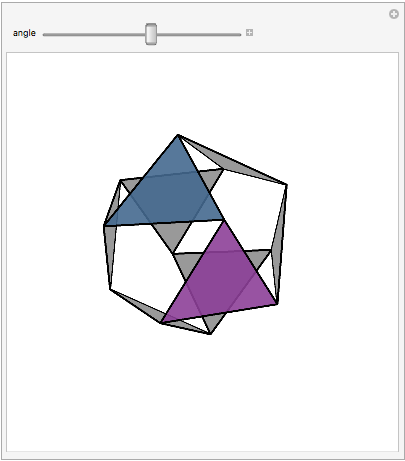
\includegraphics[width=1.5in]{imagesattalk/fccframe030.png} 
\end{figure}}
\only<2>{
\begin{figure}[htbp] %  figure placement: here, top, bottom, or page
   \centering
   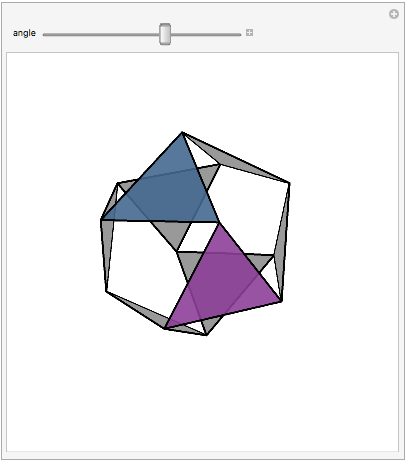
\includegraphics[width=1.5in]{imagesattalk/fccframe036.png} 
\end{figure}}
\only<3>{
\begin{figure}[htbp] %  figure placement: here, top, bottom, or page
   \centering
   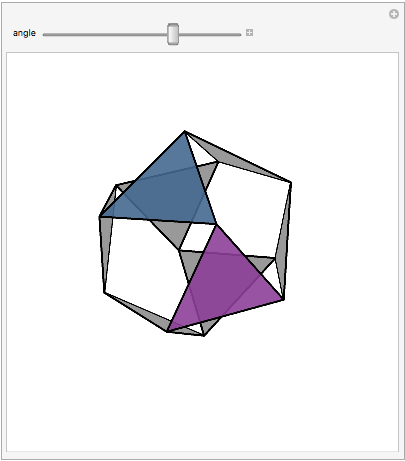
\includegraphics[width=1.5in]{imagesattalk/fccframe038.png} 
\end{figure}}
\only<4>{
\begin{figure}[htbp] %  figure placement: here, top, bottom, or page
   \centering
   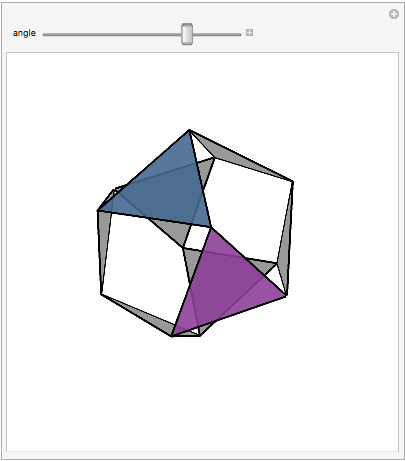
\includegraphics[width=1.5in]{imagesattalk/fccframe040.png} 
\end{figure}}
\only<5>{
\begin{figure}[htbp] %  figure placement: here, top, bottom, or page
   \centering
   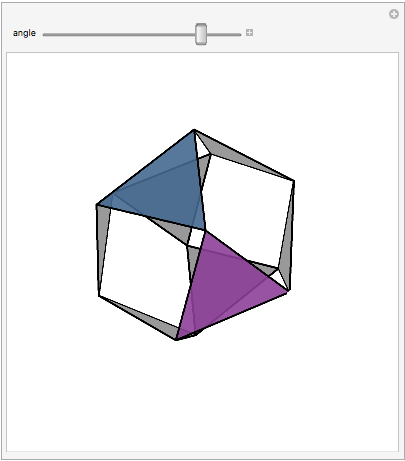
\includegraphics[width=1.5in]{imagesattalk/fccframe042.png} 
\end{figure}}
\only<6>{
\begin{figure}[htbp] %  figure placement: here, top, bottom, or page
   \centering
   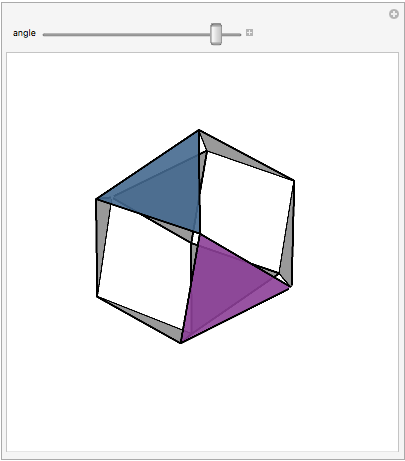
\includegraphics[width=1.5in]{imagesattalk/fccframe044.png} 
\end{figure}}
\only<7>{
\begin{figure}[htbp] %  figure placement: here, top, bottom, or page
   \centering
   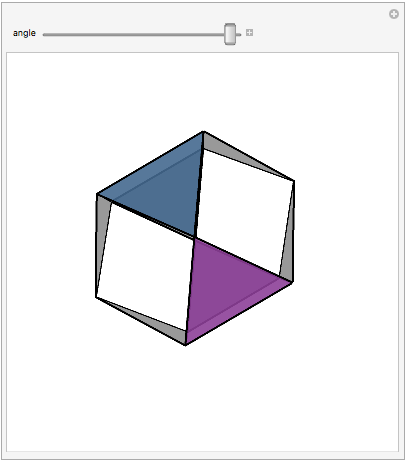
\includegraphics[width=1.5in]{imagesattalk/fccframe046.png} 
\end{figure}}


Connects icosahedron to FCC.

\end{column}


\begin{column}{.40\textwidth}
\vspace{-1cm}
\begin{figure}[htbp] %  figure placement: here, top, bottom, or page
   \centering
   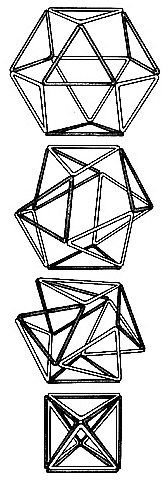
\includegraphics[width=1in]{imagesattalk/unnamed} 

\end{figure}
\end{column}
\end{columns}
}

\frame{
\frametitle{The Kagome Jitterbug}
\centering

\only<1>{
\begin{figure}[htbp] %  figure placement: here, top, bottom, or page
   \centering
   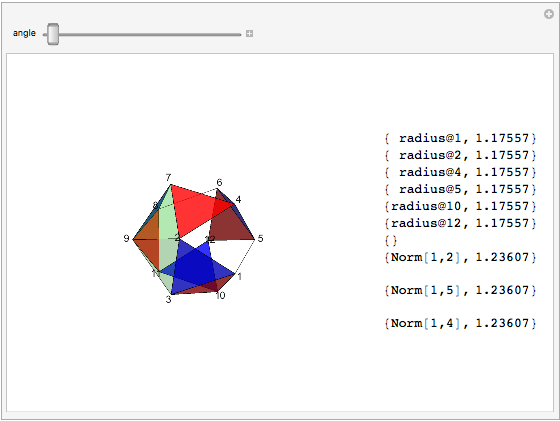
\includegraphics[width=3in]{imagesattalk/hcpframe001.png} 
\end{figure}}
\only<2>{
\begin{figure}[htbp] %  figure placement: here, top, bottom, or page
   \centering
   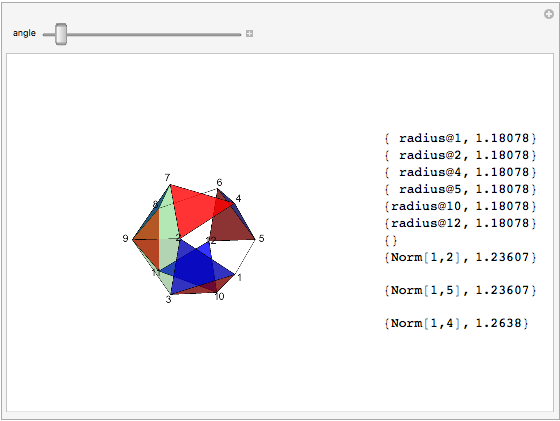
\includegraphics[width=3in]{imagesattalk/hcpframe007.png} 
\end{figure}}
\only<3>{
\begin{figure}[htbp] %  figure placement: here, top, bottom, or page
   \centering
   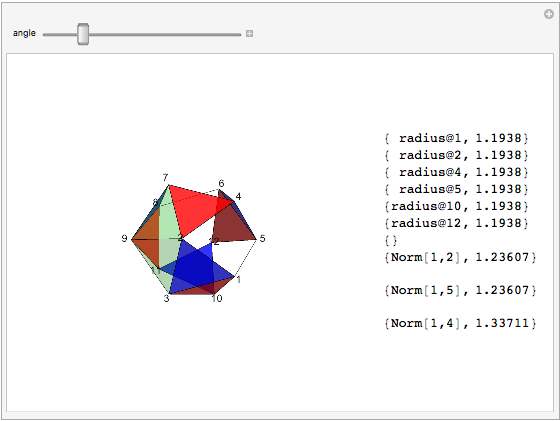
\includegraphics[width=3in]{imagesattalk/hcpframe010.png} 
\end{figure}}
\only<4>{
\begin{figure}[htbp] %  figure placement: here, top, bottom, or page
   \centering
   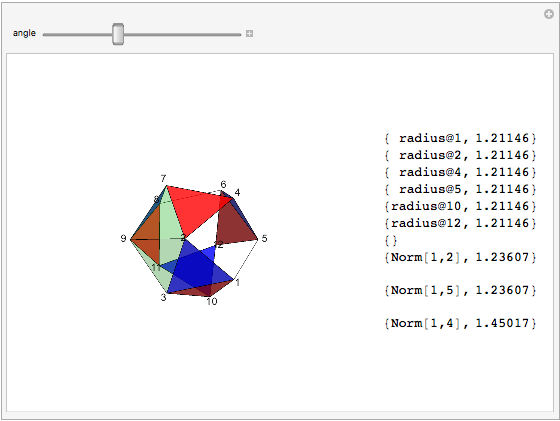
\includegraphics[width=3in]{imagesattalk/hcpframe015.png} 
\end{figure}}
\only<5>{
\begin{figure}[htbp] %  figure placement: here, top, bottom, or page
   \centering
   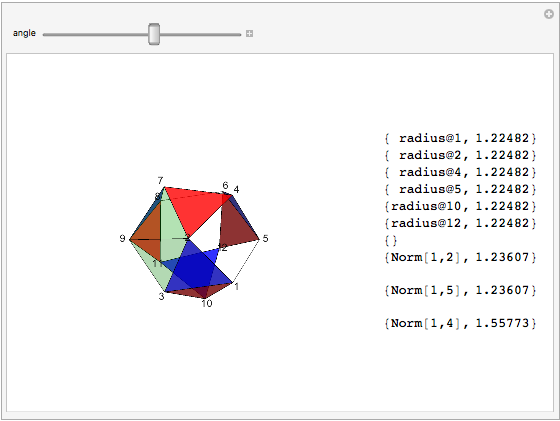
\includegraphics[width=3in]{imagesattalk/hcpframe020.png} 
\end{figure}}
\only<6>{
\begin{figure}[htbp] %  figure placement: here, top, bottom, or page
   \centering
   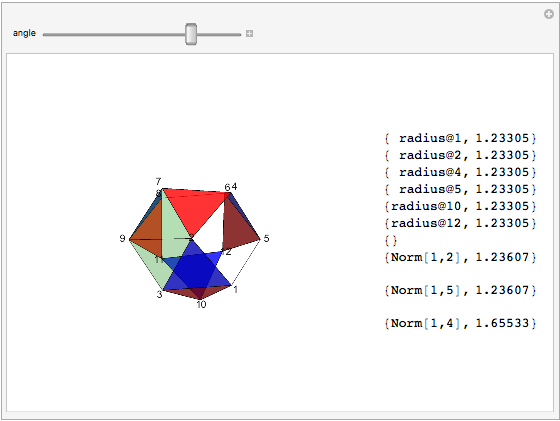
\includegraphics[width=3in]{imagesattalk/hcpframe025.png} 
\end{figure}}
\only<7>{
\begin{figure}[htbp] %  figure placement: here, top, bottom, or page
   \centering
   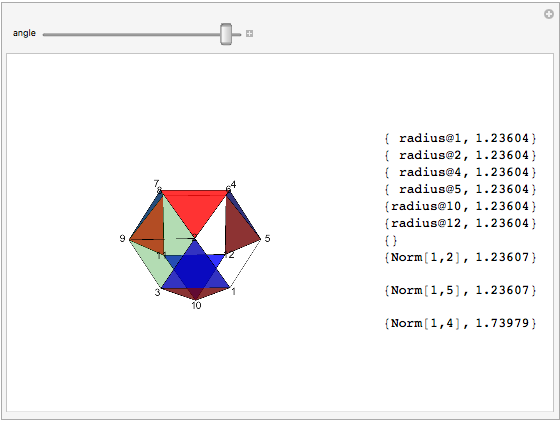
\includegraphics[width=3in]{imagesattalk/hcpframe030.png} 
\end{figure}}


Connects icosahedron to HCP.
}

\frame{
\frametitle{Motions of spheres}


\only<1>{
\begin{figure}[htbp] %  figure placement: here, top, bottom, or page
   \centering
   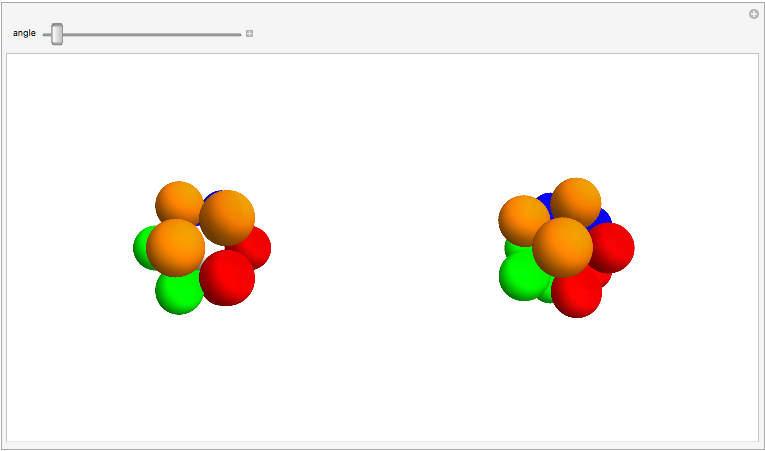
\includegraphics[width=3in]{imagesattalk/bframe025.png} 
\end{figure}}
\only<2>{
\begin{figure}[htbp] %  figure placement: here, top, bottom, or page
   \centering
   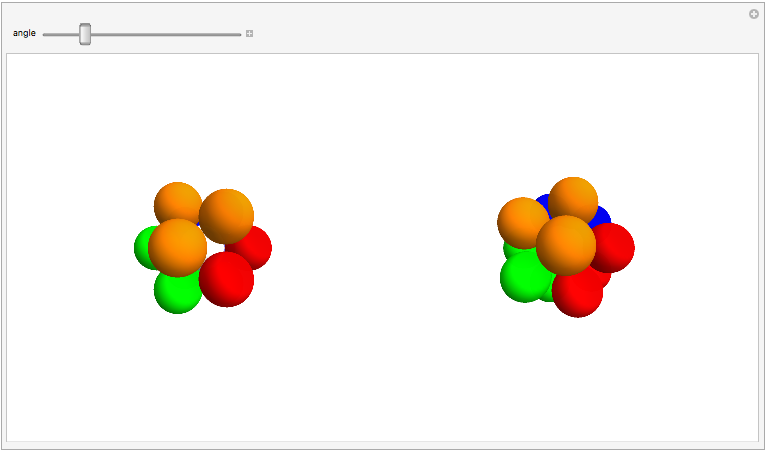
\includegraphics[width=3in]{imagesattalk/bframe030.png} 
\end{figure}}
\only<3>{
\begin{figure}[htbp] %  figure placement: here, top, bottom, or page
   \centering
   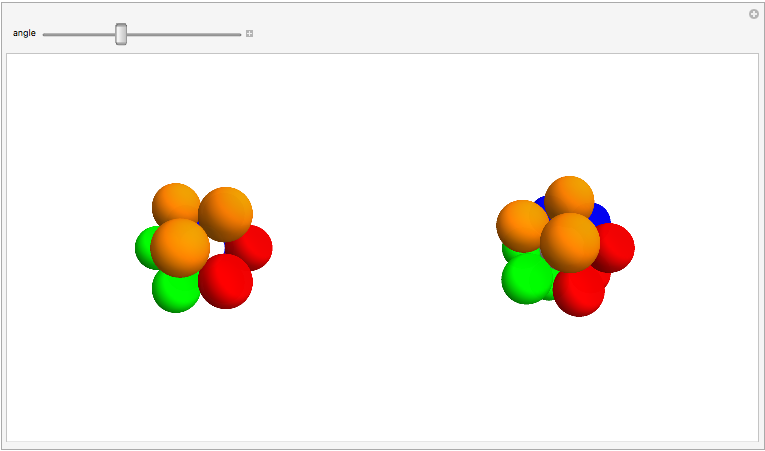
\includegraphics[width=3in]{imagesattalk/bframe035.png} 
\end{figure}}
\only<4>{
\begin{figure}[htbp] %  figure placement: here, top, bottom, or page
   \centering
   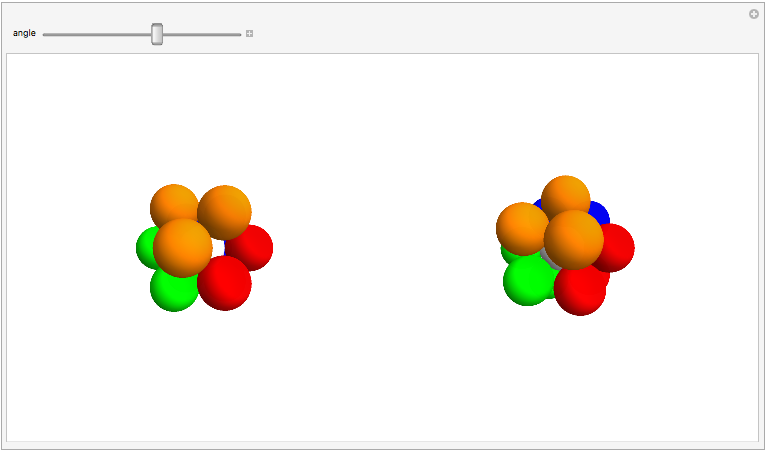
\includegraphics[width=3in]{imagesattalk/bframe040.png} 
\end{figure}}
\only<5>{
\begin{figure}[htbp] %  figure placement: here, top, bottom, or page
   \centering
   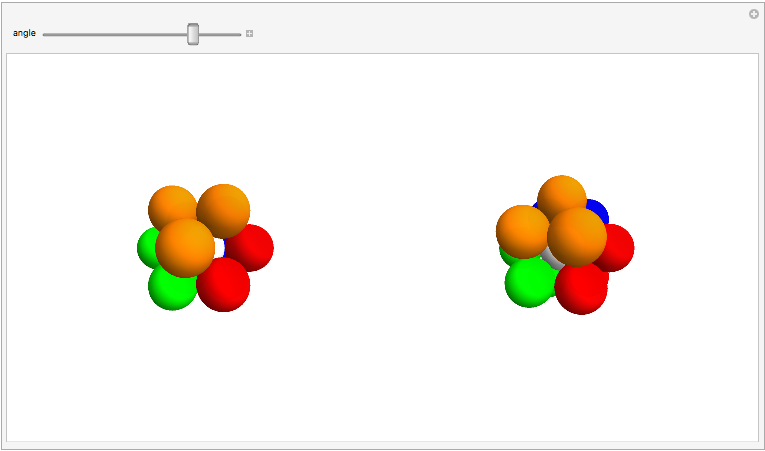
\includegraphics[width=3in]{imagesattalk/bframe045.png} 
\end{figure}}
\only<6>{
\begin{figure}[htbp] %  figure placement: here, top, bottom, or page
   \centering
   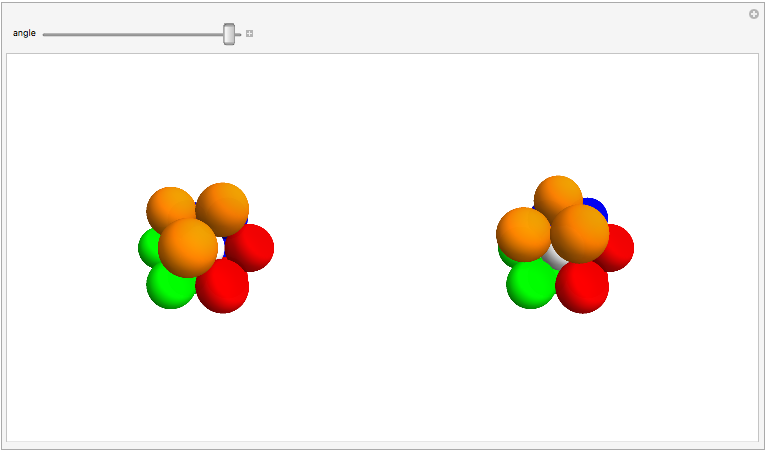
\includegraphics[width=3in]{imagesattalk/bframe050.png} 
\end{figure}}
\only<7>{
\begin{figure}[htbp] %  figure placement: here, top, bottom, or page
   \centering
   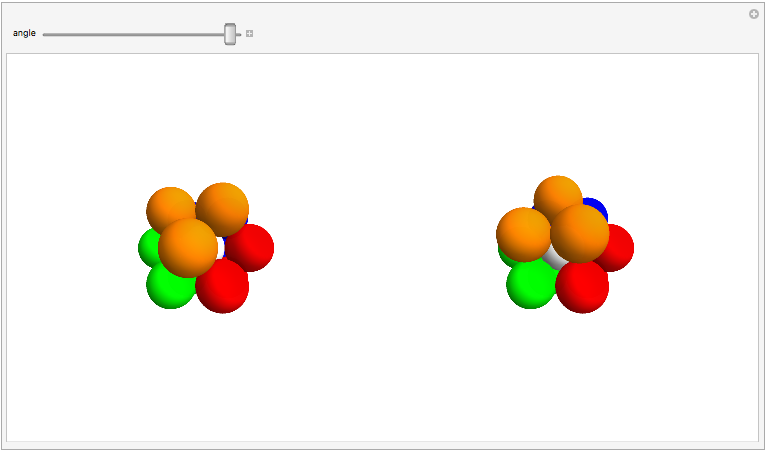
\includegraphics[width=3in]{imagesattalk/bframe055.png} 
\end{figure}}
\only<8>{
\begin{figure}[htbp] %  figure placement: here, top, bottom, or page
   \centering
   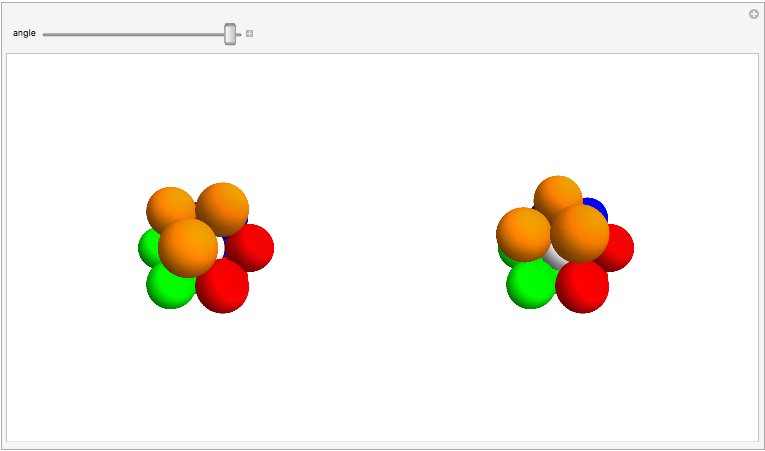
\includegraphics[width=3in]{imagesattalk/bframe060.png} 
\end{figure}}


}



\frame{
\frametitle{Motions of spheres}
The assertion that there are exactly three arrangements is \emph{false}. There \emph{is} an underlying kernel of truth in this statement: each of three the arrangements above is ``remarkable''.
\newline

\onslide<2,3>{
\begin{question}[Conway and Sloane] What rearrangements of $12$ unit spheres are possible via motions maintaining contact with the central unit sphere? \end{question}\hspace{0cm}\newline}
\onslide<3>{
They demonstrate that within the component of configuration space of $12$ unit spheres connected to the icosahedron, arbitrary permutations of all $12$ touching spheres are possible. }
}

\frame{
\frametitle{An icosahedral ``Rubik's cube"}

\begin{columns}[t]
\begin{column}{.45\textwidth}
The equatorial spheres can be moved towards poles and can be rotated to form half-geodesic graphs, like the bars of a birdcage.

\end{column}
\begin{column}{.45\textwidth}
\vspace{-1.5cm}
\begin{figure}[htbp] %  figure placement: here, top, bottom, or page
   \centering
 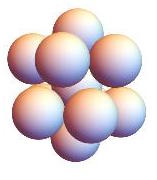
\includegraphics[width=1in]{imagesattalk/rubik1.jpg} 
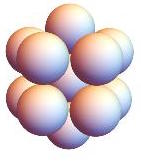
\includegraphics[width=1in]{imagesattalk/rubik2.jpg} 
\end{figure}
\end{column}
\end{columns}
\hspace{0cm}
\newline\newline
The rings of five freely rotate relative to each other.  Conway and Sloane note the conjugation action gives all $5$-cycles. \newline
\begin{remark}\centering
The fact that all $5$-cycles can be produced this way is nontrivial.\\ All $5$-cycles generate $A_{12}$.
\end{remark}
}










\frame{
\frametitle{Hidden Symmetry}

\begin{columns}[t]
\vspace{-.5cm}
\begin{column}{.50\textwidth}
The Jitterbug gives a smooth motion from the icosahedron to the FCC configuration. This has an axis of $4$-fold symmetry and $3$ layers. Therefore conjugating a rotation with the Jitterbug describes an odd permutation.  
\newline\newline
With the icosahedral Rubik's cube, this generates all of $S_{12}$.

\begin{theorem}[Conway and Sloane]
Spheres at the vertices of a regular icosahedron can be arbitrarily permuted.
\end{theorem}
\end{column}

\begin{column}{.50\textwidth}


\begin{figure}[htbp] %  figure placement: here, top, bottom, or page
   \centering
   \includegraphics[width=2in]{imagesattalk/fcc2.png} 

\end{figure}

\end{column}
\end{columns}

}



\frame{
\frametitle{Higher critical radii for $12$ points}

\begin{columns}[t]
\begin{column}{.50\textwidth}
For $1+\epsilon>r>1$,it is possible to get at least $A_{12}$.\newline

In the ``Rubik's cube", one can perturb $4$ vertical pairs to so the radius can be increased slightly and $1$ pair passes. This yields a different type of configuration, but the same idea applies.
\onslide<4>{
\begin{remark}
$\operatorname{Conf}(12,r)$ near maximal $\,r$ is a set with $12!$ components and $\operatorname{Conf}(12,r)$ just above radius $\,1$ connects them. There must be a critical value above $\,r=1$.
\end{remark}}
\end{column}

\begin{column}{.40\textwidth}

\only<1>{\vspace{0cm}

\begin{figure}[htbp] %  figure placement: here, top, bottom, or page
\includegraphics[width=1in]{imagesattalk/rubik2.jpg} 
\end{figure}
\begin{figure}[htbp] %  figure placement: here, top, bottom, or page
   \centering
   \includegraphics[width=1in]{imagesattalk/rings.jpeg} 
\end{figure}

}


\only<2,3,4>{
\vspace{-2em}
\begin{figure}[htbp] %  figure placement: here, top, bottom, or page
   \centering
   \includegraphics[width=1in]{imagesattalk/move2} 
\end{figure}
\vspace{-.5em}

\begin{figure}[htbp] %  figure placement: here, top, bottom, or page
   \centering
   \includegraphics[width=1in]{imagesattalk/move3} 
\end{figure}
\vspace{-.5em}

\begin{figure}[htbp] %  figure placement: here, top, bottom, or page
   \centering
   \includegraphics[width=1in]{imagesattalk/move4} 
\end{figure}}
\vspace{-.5em}
\only<3,4>{
\begin{figure}[htbp] %  figure placement: here, top, bottom, or page
   \centering
   \includegraphics[width=1in]{imagesattalk/move5} 
\end{figure}
\vspace{-.5em}

\begin{figure}[htbp] %  figure placement: here, top, bottom, or page
   \centering
   \includegraphics[width=1in]{imagesattalk/move6} 
\end{figure}}

\end{column}
\end{columns}

}


\frame{
\frametitle{A remark on random jammed packings}


\movie[]{:(}{water.mov}


}


\frame{
\frametitle{Thank you for your attention!}
 
\centering
wkusner.github.io
  
Supported by Austrian Science Fund (FWF) Project 5503 

}






\end{document}

